\documentclass[unicode]{scutthesis}

\usepackage[unicode=false,bookmarks=true,bookmarksnumbered=true,bookmarksopen=false,
 breaklinks=false,pdfborder={0 0 1},backref=false,colorlinks=true]
 {hyperref}
 
\hypersetup{pdftitle={博士论文标题},
 pdfauthor={你的名字},
 pdfsubject={华南理工大学博士学位论文},
 pdfkeywords={关键字1, 关键字2},
 linkcolor=blue, anchorcolor=black, citecolor=olive, filecolor=magenta, menucolor=red, urlcolor=magenta, pdfstartview=FitH}
 
\begin{document}
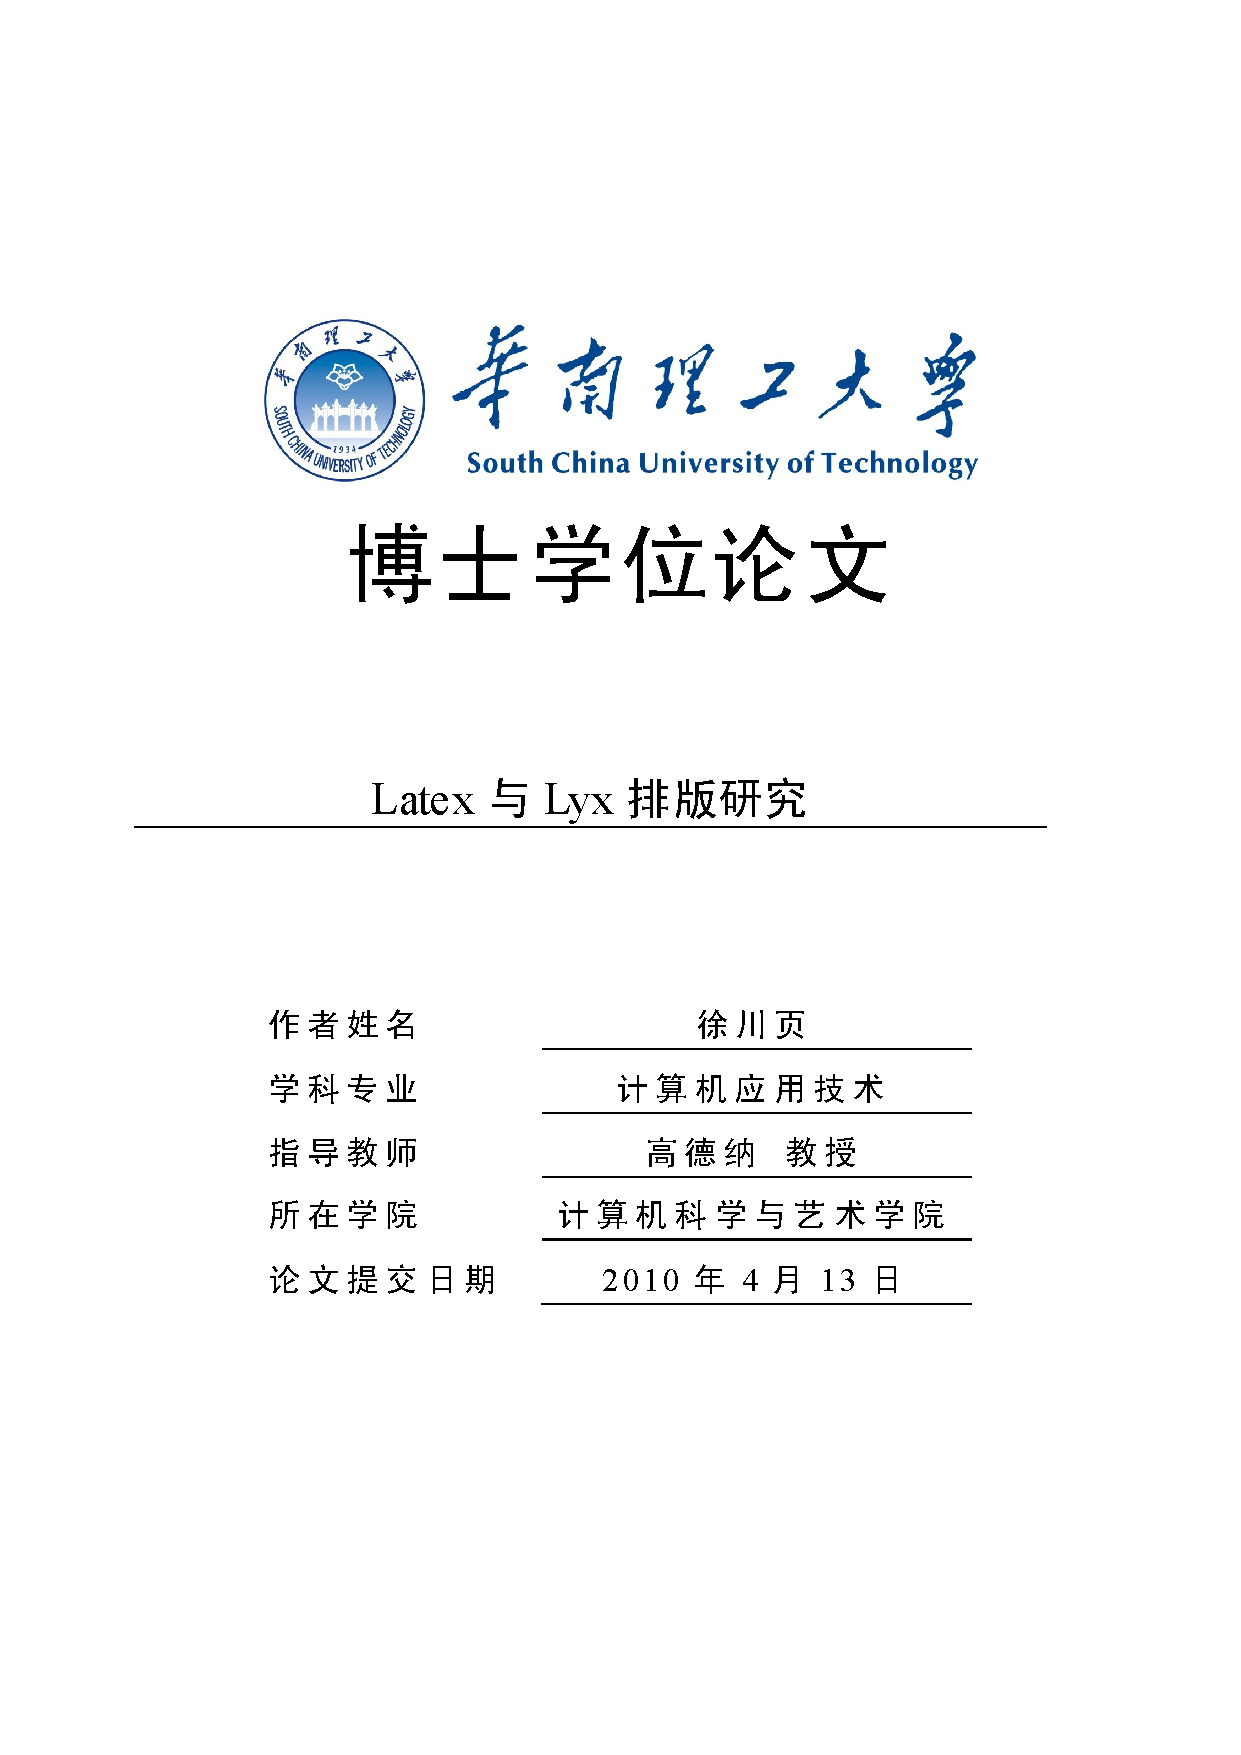
\includepdf[pages=-]{thesis_cover.pdf}%包含pdf头文件

\frontmatter

\begin{abstractCn}
本文用于测试scutthese.cls的使用,主要包括xelatex是否正常可调用,中文字体是否显示之前,pdf标签是否正确显示。
\end{abstractCn}
\keywordsCn{\LaTeX{};排版;论文}

\begin{abstractEn}
This article tests the usage of scutthese.cls \LaTeX{} typesetting.
\end{abstractEn}
\keywordsEn{\LaTeX{};  Typesetting; Paper}


\tableofcontents{}
 
\mainmatter

\chapter{绪论}
Tex排版\cite{knuth1986thetexbook}是由Knuth最早发明,后来人们对其扩展了大量宏包以增强其功能,而且设计了多种不同的Tex专业引擎,其中内置了许多常用的Tex宏包,如\LaTeX{}\cite{goossens1994thelatex};内核不同的新TEX引擎,如XeTex(包含LaTex宏包的称为XeLaTex),它支持支持UTF-8文档编码而以pdf格式输出。

XeTex引擎使用xeCJK宏包支持中文排版,大大方便了中日韩语言用户排名。我们自定义了scutthesis.cls模板库,它是基于latex/base/book.cls进行文章结构布局,并调用了xelatex/xecjk/xeCJK.sty宏包,以UTF-8方式支持中文显示。scutthesis.cls模板库是一套“华南理工大学博士学位论文”模板。

\section{English}
Test English section name.

\section{中文}
测试中文section的标题名,中文文献引用\cite{cnproceed, wang_model_2009}.


\chapter{结论}
我们测试了自定义的scutthesis.cls模板库的中英文显示效果。使用了XeLaTex而不是\LaTeX{}的Tex编译引擎。
正确安装XeTex(XeLaTex)后,此文正常编译后为pdf文件,其的中英文内容、标题和pdf标题都应该显示正常。


\backmatter

\bibliographystyle{scutthesis}
\bibliography{scutthesis}

\pagestyle{appendix_style}

\appendix{附录}
\section{Ubuntu Linux系统下中文字体的安装}
\label{sec:ubuntuzhfont}
整个过程分为两部分:得到中文字体文件和安装设置。

常用中文字体有三套:

1. winfonts(微软的六种中易字体,包括宋体、黑体、楷书、仿宋、隶书、幼圆),

2. adobefonts(Adobe 的四套字体,包括 Adobe Song Std、Adobe Heiti Std、Adobe
Fangsong Std、Adobe Kaiti Std)

3. Ubuntu开源的文泉字体
CTex宏库默认支持winfonts和adboefonts。因此要在linux系统下使用Ctex宏库最好是安装这些字库之一。

\section{Texlive的安装}

\label{sec:texlive_install}

Texlive是TEX的一个集成发行包,相关介绍见http://tug.org/texlive/doc/texlive-zh-cn/。其主要过程包括:预设置、下载安装和测试调用。建议用GUI方式安装:

sudo apt-get install perl-tk 

到http://tug.org/texlive/acquire-netinstall.html页面下载 install-tl在线安装前端程序.


\appendix{攻读博士学位期间取得的研究成果}

已发表(包括已接受待发表)的论文,以及已投稿、或已成文打算投稿、或拟成文投稿的论文情况(只填写与学位论文内容相关的部分):

\begin{table}
\begin{longtable}{|>{\centering}m{0.5cm}|>{\centering}m{2.3cm}|>{\centering}m{3.5cm}|>{\centering}m{2.6cm}|>{\centering}m{2cm}|>{\centering}m{1.3cm}|>{\centering}m{0.9cm}|}
\hline 
序号 & 作者(全体作者,按顺序排列) & 题 目 & 发表或投稿刊物名称、级别 & 发表的卷期、年月、页码 & 相当于学位论文的哪一部分(章、节) & 被索引收录情况\tabularnewline
\hline 
1 & 作者名 & 论文题目1 & 刊物名 & 发表时间 & 第2章 & SCI\tabularnewline
\hline 
2 & 作者名 & 论文题目2 & 刊物名 & 发表时间 & 第3章 & SCI\tabularnewline
\hline 
 &  &  &  &  &  & \tabularnewline
\hline 
 &  &  &  &  &  & \tabularnewline
\hline 
 &  &  &  &  &  & \tabularnewline
\hline 
 &  &  &  &  &  & \tabularnewline
\hline 
\end{longtable}
\end{table}



\appendix{致谢}

首先感谢国家,感谢党;再感谢导师对我的指导,最后感谢父母亲对我的期望!

同时感谢华工校内外多位同学对该模板的测试和提供的改进。

\begin{minipage}[t]{0.8\columnwidth}%
\begin{flushright}
徐顺 
\par\end{flushright}

\begin{flushright}
\today
\par\end{flushright}%
\end{minipage}

\end{document}
